\documentclass[11]{article}
\usepackage[margin=1in]{geometry}
\usepackage{amsfonts,amsmath,amssymb}
\usepackage{fancyhdr}
\usepackage{graphicx}
\usepackage{float}
\usepackage{transparent}
\usepackage{eso-pic}
\usepackage[colorlinks,linkcolor={blue}]{hyperref}



\usepackage{listings}
\usepackage{color}


\definecolor{dkgreen}{rgb}{0,0.6,0}
\definecolor{gray}{rgb}{0.5,0.5,0.5}
\definecolor{mauve}{rgb}{0.58,0,0.82}

\lstset{frame=tb,
  language=Java,
  aboveskip=3mm,
  belowskip=3mm,
  showstringspaces=false,
  columns=flexible,
  basicstyle={\small\ttfamily},
  numbers=none,
  numberstyle=\tiny\color{gray},
  keywordstyle=\color{blue},
  commentstyle=\color{dkgreen},
  stringstyle=\color{mauve},
  breaklines=true,
  breakatwhitespace=true,
  tabsize=3
}



\newcommand\BackgroundPic{%
\put(0,0){%
\parbox[b][\paperheight]{\paperwidth}{%
\vfill
\centering
{\transparent{0.3} 
\includegraphics[width=\paperwidth,height=\paperheight,%
keepaspectratio]{background.jpg}}%
\vfill
}}}

\AddToShipoutPicture*{\BackgroundPic}

\pagestyle{fancy}
\fancyhead{}
\fancyfoot{}
\fancyhead[L]{\slshape \MakeUppercase{Notes}}
\fancyfoot[C]{\thepage}
%\renewcommand{\headrulewidth}{0pt}
\renewcommand{\footrulewidth}{0pt}

\parindent 0ex
\renewcommand{\baselinestretch}{1.5}

\begin{document}
\begin{titlepage}
\begin{center}
\vspace{1cm}
\Large{\textbf{Computer Science 101: Introduction to Java and Algorithms}}\\
\vfill
\line(1,0){400}\\
\huge{\textbf{Section 4: Arrays}}\\
\line(1,0){400}\\
\vfill
Erudition Labs\\
Computer Science 101: Introduction to Java and Algorithms\\
\today\\
\end{center}
\end{titlepage}

\tableofcontents
\thispagestyle{empty}
\clearpage
\setcounter{page}{1}

\section{Terminology}
\begin{itemize}
  \item \textbf{\textit{Memory}} --
  Memory is where all the action happens. Many people often refer to it as storage space although that is not entirely true. When programmers talk of memory, we are talking about addressable memory. This means memory that computers can create addresses for and thus use. Memory is NOT hard drive space. It is RAM. The amount of memory you have depends on two things. The amount of RAM you have and the operating systems you are using (eg. 32 bit windows vs 64 bit windows). With 32 bit systems, you are limited to 4 GB of ram where as 64 bit machines are (theoretically since we haven`t done it) limited to 16.8 million terabytes of RAM. Everything happens in your memory. When you start up your computer, windows (or mac, linux, android, IOS...whatever) gets loaded into memory. Whenever you launch a program, it gets loaded into memory. Pretty much whenever you do anything on a computer, it`s done in memory. As a programmer, you generally deal with two types of memory, heap and stack. Refer to \autoref{sec:heap} to lean more about heap vs stack.

  
  \item \textbf{\textit{Data Structure}} -- Data structures is basically a term to describe a way of organizing data. We create certain rules for how we store and organize data so that we can take advantage of its organization when performing operations like insertion, retrieval, and searching. Some example data structures are arrays, linked lists, binary trees, hash maps and vectors. Feel free to look any up if you are curious. One of the simplest to understand is the linked list.
  
  \item \textbf{\textit{Collections}} -- In many programming languages we often come across the terms collections and containers. In Java, we only deal with collections. A collection is a way of grouping data together under the same name. I would recommend \url{<https://www.geeksforgeeks.org/collections-in-java-2/>} if you are curious about more.
  
  \item \textbf{\textit{Array}} -- A collection of data elements of the same type stored in a contiguous chunk of memory.
  
  \item \textbf{\textit{Elements of an array}} -- We use this phrase to talk about all of the pieces of data stored in an array.
  
  \item \textbf{\textit{Iterate over an array (loop over an array)}} -- We use these phrases when we are talking about using one of the loops, like a for or while loop, to look at each element in an array (one each iteration of the loop).
  
  \item \textbf{\textit{Random access}} -- This means we can access an arbitrary piece of memory. In reference to arrays, it means that we can access any arbitrary element in an array as long as it exists. You won`t hear this term too much until you learn about algorithm efficiency.
  
  \item \textbf{\textit{Index}} -- The position of something, often in an array-like collection. In reference to arrays, the index is the position that an element is stored at in the array.
  
  \item \textbf{\textit{Index into an array}} -- We are using the index (aka the position of an element in an array) to get the value of the element at that position in the array.
  
  \item \textbf{\textit{Allocate memory}} -- Whenever we need create variables, the compiler looks at the type of variable  (int, float etc) and sets aside the right amount of memory to store values of that type (aka allocate memory). However, in the case of things like arrays and object (more on objects later), the programmer need to allocate the memory. Basically, any time you use the ``new`` keyword, you are allocating memory for that type to store the values.
  
\end{itemize}
\section{Pre-Chapter}
\subsection{Heap and Stack Memory(Over Simplified)}
\label{sec:heap}

\subsection{The ``new`` keyword}
\subsection{Declaration vs. Initialization}
\section{Arrays (Video Series Lecture 20 and 21)}
This section introduces Arrays, which is a data structure that stores collections of elements. What is a data structure? Well a data structure is just a way organizing data by following certain rules when we store and retrieve it. By doing this, we can take advantage of the way the data is organized to make efficient algorithms. Some data structures are better at some things than others. It all depends on what you need to do. So when you take a data structures class (or look into it yourself) you will learn about different data structures (aka different ways of organizing data), their rules, their advantages, disadvantages and their best use cases.\\

For example, if your program is going to be doing a lot of retrieving, there are data structures that are great for that. If you need to do a lot of saving or insertions, we have great data structures for that too, but those might also not be the best for retrieving. There are often trade-offs when using them and it is up to the programmer to decide which ones are best for your task. For now, you don`t really need to know what a data structure is other than it`s a way if organizing data. If you are taking computer science classes, then there are entire classes dedicated to that topic. All you need to know right now is that an array is used to store a collection of things of the same type and are extremely good for random access (meaning I can get any arbitrary piece of data at any time efficiently as long as I know where it is at in the array).
\subsection{What does an Array Look Like?}
Arrays are contiguous chunks of memory. And they MUST be contiguous due to how we access the data. I will talk about that more later. Usually when we try to visualize and conceptualize what an array is, we draw it like this:\\

\begin{figure}[H]
	\centering
	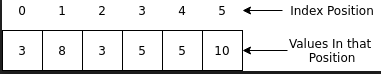
\includegraphics[scale=0.5]{arrays1.png}
	\caption{Image from Lecture}
\end{figure}

Imagine, if you will, having a bunch of variables of the same type under one name. This is essentially what an array is. So if you need to store a collection of integers, you can declare one array to store them instead of declaring a bunch of different variables. If you look at the table, the top row corresponds to the index position of the array. The index is simply where that particular piece of data is stored at in the array. Also note that we refer to these ``pieces of data`` as elements. For example, if we look at the table above, we can see that $8$ is an element of that array at index position $1$. \\

Notice that we start counting from $0$. The $0$th element is actually the first element in the array. Next, you can see all the boxes (aka the elements). Think of each box as a variable that you don`t have to name that stores a value. So in the image, we have an array of size $6$ that stores $6$ integers.\\

\subsection{Declaring/Initializing an Array}
We can declare an array just like we declare any other variable, in the form of
\begin{lstlisting}
int myArray[];
\end{lstlisting}
Now that we have declared the array, the compiler knows what we are talking about, but we cannot use it. Before we can use an array, we must initialize it with a size. We do that with the ``new`` keyword.

\begin{lstlisting}
int myArray[];
myArray = new int[10];
\end{lstlisting}
Java guarantees that the elements in the array allocated using new will automatically be initialized to zero (for numeric types), false (for boolean), or null (for when you learn about objects). Why does this matter? Because bad things happen when we try to access memory that has ``nothing`` in it. We will talk about it further in the ``Gotchas``  \autoref{sec:gotchas}. \\

Now lets briefly look at other common ways to declare and initialize arrays.

\begin{lstlisting}
int myArray[]; //declare
myArray = new int[10]; //initialize separately
//----------------------------------------

int myArray[] = new int[10] //initialize in one line
//----------------------------------------

int size = 5;
int myArray[] = new int[size]; //use variable for size
//----------------------------------------

int size = 5;
int myArray[]; //declare
myArray = new int[size]; //initialize separately

//-------------------------------------
int[] myArray = new int[] {5, 7, 3, 9, 10, 15, 27};
//create array and assign values to each position
\end{lstlisting}

\subsection{Accessing Elements}
To access elements, we need to know the position of the element in the array. The best way to see what I`m talking about is to let the code talk.

\begin{lstlisting}
class Main {
  public static void main(String[] args) {
    String myArray[] = new String[2]; //create array of size 2
    //access array using index
    myArray[0] = "hello"; // first element
    myArray[1] = "world"; // secodn element

    System.out.println(myArray[0] + " " + myArray[1]);
  }
}
\end{lstlisting}

At the beginning of the code, we create a String array of size two. So our array would look like this:
\begin{center}
	\begin{tabular}{ | c | c | } \hline
 	null & null  \\   \hline
	\end{tabular}
\end{center}

The next line, we access the first element of the array and set it equal to `` hello``. So now our array looks like this:

\begin{center}
	\begin{tabular}{ | c | c | } \hline
 	``hello`` & null  \\   \hline
	\end{tabular}
\end{center}

Then we do the next index position and set it to ``world``. 

\begin{center}
	\begin{tabular}{ | c | c | } \hline
 	``hello`` & ``world``  \\   \hline
	\end{tabular}
\end{center}

Finally we just print the the element at index $0$ concatenated with an empty space (so we have a space between out words so it looks like ``hello world`` instead of ``helloworld``) which is also concatenated with ``world``. So the output of this program is ``hello world``.	

\section{Looping Over Arrays (Video Series Lecture 22 and 23)}
Often times we need a way of looking at all of the elements in a given array (perhaps you are searching for an element for example or you would like to print out all of the elements). You can use the different types of loops to loop over the array. The most common loop used is the for loop since it maintains the current index with the current iteration. For example, If we want to search for an element in an array and print it out, we could do something like:

\begin{lstlisting}
class Main {
  public static void main(String[] args) {
    int[] myArray = new int[] {5, 7, 3, 9, 10, 15, 27}; //create array with values
    for(int i=0; i<myArray.length; i++) {
      if(myArray[i] == 9) {
        System.out.println("We found a 9 at array position " + i);
      }
    }
  }
}
\end{lstlisting}
In this code, we create an array and set values. We use the for loop to iterate until the variable $i$ reaches the number of elements (aka we loop to the end). Then we use variable $i$ to index into the array to get the value at that position and compare it to $9$. When the if statement evaluates to true, we execute the print statement. So the output of this code is ``We found a 9 at array position $3$``. If you look at the array we created, starting from $0$, you will see that there is a $9$ at position $3$ of the array.\\

Now let`s we want to print out all of the elements in the array? Can we simply do this:

\begin{lstlisting}
class Main {
  public static void main(String[] args) {
    int[] myArray = new int[] {5, 7, 3, 9, 10, 15, 27}; //create array with values
	System.out.println(myArray); // Can we do this? NOOOOOOO
  }
}
\end{lstlisting}

Turns out, we cannot do this. If you were to try, your output will look something like, ``[I@4aa298b7``. What the heck is that? Well to put it simply, you can think of that as the address in memory where the array is stored.\\

So how do we print out all of the elements? Well you have to loop over each one and print it out.

\begin{lstlisting}
class Main {
  public static void main(String[] args) {
    int[] myArray = new int[] {5, 7, 3, 9, 10, 15, 27}; //create array with values
    for(int i=0; i<myArray.length; i++) {
      System.out.print(i + " ");
    }
  }
}
\end{lstlisting}

This outputs ``0 1 2 3 4 5 6``
\subsection{Increasing/Decreasing the size of an Array}
Can we take an existing array and increase or decrease it`s size? No. Sooooooo, now what? If you need to increase of decrease the size of an array, then you need to initialize a new array and use a loop to copy all of your elements over into the new array and assign your old array to your new array. Let`s let the code talk.

\begin{lstlisting}
class Main {
  public static void main(String[] args) {
    double myArray[] = new double[10]; //create array of size 10

    //OH NO, I ran out of room!!!

    double tempBiggerArray[] = new double[myArray.length * 2]; //new bigger temp array twice the size of my other array
    for(int i=0; i<myArray.length; i++) { //loop over old array of size 10
      tempBiggerArray[i] = myArray[i]; //copy over each element
    }
      myArray = tempBiggerArray; // now myArray has size 20
  }
}
\end{lstlisting}

As you can imagine, this seems like it isn`t an efficient thing to do every time you need more space. This is a limitation of arrays. They must be initialized with a fixed length. And the size must be known at the time of initialization. This means that I must know how big I need my array to be so that I can create one big enough.
\section{2D Arrays (Video Series Lecture 24 and 25)}
\section{Sorting Arrays: Insertion Sort Algorithm (Video Series Lecture 26 and 27)}
\section{Gotchas with Arrays}
\label{sec:gotchas}



\end{document}